\date{}
\title{}
\date{}
\begin{document}
\begin{frame}
    \titlepage
\end{frame}


\makeatletter
\newenvironment<>{btHighlight}[1][]
{\begin{onlyenv}#2\begingroup\tikzset{bt@Highlight@par/.style={#1}}\begin{lrbox}{\@tempboxa}}
{\end{lrbox}\bt@HL@box[bt@Highlight@par]{\@tempboxa}\endgroup\end{onlyenv}}

\newcommand<>\btHL[1][]{%
  \only#2{\begin{btHighlight}[#1]\bgroup\aftergroup\bt@HL@endenv}%
}
\def\bt@HL@endenv{%
  \end{btHighlight}%   
  \egroup %
}
\tikzset{
    btHLbox/.style={
        fill=red!30,outer sep=0pt,inner xsep=1pt, inner ysep=0pt, rounded corners=3pt
    },
}
\newcommand{\bt@HL@box}[2][]{%
  \tikz[#1]{%
    \pgfpathrectangle{\pgfpoint{1pt}{0pt}}{\pgfpoint{\wd #2}{\ht #2}}%
    \pgfusepath{use as bounding box}%
    \node[text width={},draw=none,anchor=base west, btHLbox, minimum height=\ht\strutbox+1pt,#1]{\raisebox{1pt}{\strut}\strut\usebox{#2}};
  }%
}

\lst@CCPutMacro
    \lst@ProcessOther {"2A}{%
      \lst@ttfamily 
         {\raisebox{2pt}{*}}% used with ttfamily
         {\raisebox{2pt}{*}}}% used with other fonts
    \@empty\z@\@empty

\lstdefinelanguage
   [x8664gas]{Assembler}     % add a "x64" dialect of Assembler
   [x86masm]{Assembler} % based on the "x86masm" dialect
   % with these extra keywords:
   {morekeywords={CDQE,CQO,CMPSQ,CMPXCHG16B,JRCXZ,LODSQ,MOVSXD,%
                  POPFQ,PUSHFQ,SCASQ,STOSQ,IRETQ,RDTSCP,SWAPGS,.TEXT,.STRING,.ASCIZ,%
                  BEQ,LW,SW,LB,SB,ADDIU,J,BEQZ,BNEZ,BNE,%
                  MOVUPD,MULPD,MOVSD,MULSD,%
                  SHLADD,MOV,CMP.LT,TBIT.NZ,BR.RET.SPTK.MANY,%
                  ADDQ,POPQ,PUSHQ,RRMOVQ,MRMOVQ,RMMOVQ,IRMOVQ,%
                  <-,LL,SC,ADDI,ADDL,VMOVDQA,ADDQ,CMPL,JB,JBE,MOVL,CLTQ,%
                  MOVW,PUSHW,MOV,ADD,SUB,INT,PUSH,MOV,ADD,REP,MOVSB,%
                  TESTQ,CMPQ,MOVL,MOVQ,ADDQ,JMPQ,XORQ,%
                  LEAQ,LEAL,LEA,RETQ,RET,POPL,POPW,PUSHL,PUSHW,%
                  LEAW,%
                  SUBQ,SYSCALL,.ASCII,CALLQ,MOVSLQ,JMP,ANDQ,SHRQ,MOVB,INCQ,TESTL,XORL,%
                  SHRL,LEAL,SARL,SUBL,IMULL,IMULQ,MOVDQU,PADDD,XORL,%
                  MOVZBL,MOVZB,SHRB,SRAL,SHRL,ANDL,%
                  CMOVNS,SRAL,SRAQ,MOVZBW,MOVZBQ,%
                  PADDW,PADDQ,MODUPS,MOVAPD,%
                  MOVL,RET,.GLOBL,%
		  PAUSE,LFENCE,JMP,%
                  },
    deletekeywords={eax,ebx,sp,si,cx,di,ds,cs,es,fs,dx,ax,bx,al,esi,ebp,ecx,rip,eip,edx,edi,rdi,esp},
    deletekeywords=[2]{size},
    alsoletter={\%},
    alsoother={()},
    emphstyle={\color{violet!50!black}},
    emph={\%rax,\%rbx,\%rcx,\%rdx,\%r8,\%r9,\%r10,\%r11,\%r12,\%r13,\%r14,\%r15,\%eax,\%ebx,\%sp,\%si,\%cx,\%di,\%ds,\%cs,\%es,\%fs,\%dx,\%ax,\%bx,\%al,\%esi,\%ebp,\%ecx,\%rip,\%eip,\%edx,\%edi,\%rdi,\%esp,\%rsp},
    %moreemph={eax,ebx,sp,si,cx,di,ds,cs,es,fs,dx,ax,bx,al,esi,ebp,ecx,rip,eip,edx,edi,rdi,esp},
    morecomment=[l]{\#},
    morecomment=[l]{\/\/},
    morecomment=[s]{/*}{*/},
    sensitive=false,
    keepspaces=true} % et

\lstalias[]{myasm}[x8664gas]{Assembler}

\lstdefinelanguage{JavaScript}{
  keywords={typeof, new, true, false, catch, function, return, null, catch, switch, var, if, in, while, do, else, case, break},
  ndkeywords={class, export, boolean, throw, implements, import, this},
  sensitive=false,
  comment=[l]{//},
  morecomment=[s]{/*}{*/},
  morestring=[b]',
  morestring=[b]"
}

\newcommand{\keywordstyle}{\sourcecodeprolight\bfseries\color{blue!30!black}}
\newcommand{\stringstyle}{\color{blue!20!black}\ttfamily}

\lstset{
    language=C,
    basicstyle=\sourcecodepro\EmptyMapping,
    escapechar=`,
    keywordstyle=\keywordstyle\EmptyMapping,
    identifierstyle=\sourcecodepro\EmptyMapping,
    numberstyle=\small\color{black!70},
    commentstyle=\color{red!60!black}\ttfamily\itshape,
    stringstyle=\color{blue!20!black}\ttfamily,
    ndkeywordstyle=\bfseries\color{blue!30!black},
    upquote=true,
}



\lstdefinestyle{medium}{
    basicstyle=\sourcecodepro\EmptyMapping\fontsize{12}{13}\selectfont,
    keywordstyle=\sourcecodepro\EmptyMapping\fontsize{12}{13}\selectfont\keywordstyle,
}

\lstdefinestyle{small}{
    basicstyle=\sourcecodepro\EmptyMapping\small,
    keywordstyle=\sourcecodepro\EmptyMapping\small\keywordstyle,
}

\lstdefinestyle{smaller}{
    basicstyle=\sourcecodepro\EmptyMapping\fontsize{11}{12}\selectfont,
    keywordstyle=\sourcecodepro\EmptyMapping\fontsize{11}{12}\selectfont\keywordstyle,
}

\lstdefinestyle{size105}{
    basicstyle=\sourcecodepro\EmptyMapping\fontsize{10.5}{11.5}\selectfont,
    keywordstyle=\sourcecodepro\EmptyMapping\fontsize{10.5}{11.5}\selectfont\keywordstyle,
}

\lstdefinestyle{size10}{
    basicstyle=\sourcecodepro\EmptyMapping\fontsize{10}{11}\selectfont,
    keywordstyle=\sourcecodepro\EmptyMapping\fontsize{10}{11}\selectfont\keywordstyle,
}

\lstdefinestyle{size9}{
    basicstyle=\sourcecodepro\EmptyMapping\fontsize{9}{10}\selectfont,
    keywordstyle=\sourcecodepro\EmptyMapping\fontsize{9}{10}\selectfont\keywordstyle,
}
\lstdefinestyle{size8}{
    basicstyle=\sourcecodepro\EmptyMapping\fontsize{8}{9}\selectfont,
    keywordstyle=\sourcecodepro\EmptyMapping\fontsize{8}{9}\selectfont\keywordstyle,
}



\lstdefinestyle{script}{
    basicstyle=\sourcecodepro\EmptyMapping\scriptsize,
    keywordstyle=\sourcecodepro\EmptyMapping\scriptsize\bfseries,
}





\begin{frame}<1>[label=stackCanHopes]{stack canary hopes}
    \begin{itemize}
    \item \myemph<2>{overwrite return address $\implies$ overwrite canary}
    \item \myemph<3>{canary is secret}
    \end{itemize}
\end{frame}




\begin{frame}{last time}
    \begin{itemize}
    \item Morris worm as example
    \item writing machine code without certain byte values
        \begin{itemize}
        \item x86-64 subset: incl. push/pop/some xor/imul
        \item can write new machine code from old machine code
        \item observation: stack is after shellcode
        \end{itemize}
    \item alternate places to put shellcode
    \item stack canaries
    \item information leaks (start)
    \end{itemize}
\end{frame}

\begin{frame}{on the quiz}
    \begin{itemize}
    \item quiz Q1 --- hooking functionality for examining list of running programs
        \begin{itemize}
        \item hooking = intercepting/manipulation use of this function
        \item can use this to tell when functionality in use --- not veyr good indication of activity
        \end{itemize}
    \item quiz Q2 --- analysis in Ghidra --- typically not running malware

    \end{itemize}
\end{frame}

\begin{frame}[fragile]{long NOP setting instructions}
    \begin{itemize}
    \item Q came up during TRICKY office hours
    \end{itemize}
\begin{Verbatim}
   1:   66 66 2e 0f 1f 84 00    data16 cs nopw 0x0(%rax,%rax,1)
   8:   00 00 00 00 
   c:   0f 1f 40 00             nopl   0x0(%rax)
\end{Verbatim}
\begin{itemize}
\item what are these instructions/why?
\item long nops recommended in Intel manuals
    \begin{itemize}
    \item 66, 2e are do-nothing prefixes
    \item 0f 1f is opcode for argument-taking nop instruction
    \item argument is (mostly) ignored, but takes up space
    \end{iitemize}
\item long nops recommended b/c more efficient to process than lots of short nops
\end{itemize}
\end{frame}

\begin{frame}{on the setting stack pointer exercise}
\end{frame}

\usetikzlibrary{decorations.pathreplacing,decorations.pathmorphing}

\begin{frame}[fragile,label=stackNonContigEx]{exercise: non-contiguous overwrites}
\begin{lstlisting}[style=small]
void vulnerable() {
  int scores[8]; bool done = false;
  while (!done) {
    cout << "Edit which score? (0 to 7) ";
    int i;
    cin >> i;
    /* Oops!
       sizeof(scores) is 4 * sizeof(int) */
    if (i < 0 || i >= sizeof(scores))
      continue;
    cout << "Set to what value?" << endl;
    cin >> scores[i];
    ...
  }
  ...
}
\end{lstlisting}
\begin{tikzpicture}[overlay,remember picture,y=1.25cm]
\begin{pgfonlayer}{fg}
\coordinate (stack tl) at ([xshift=-4cm,yshift=-1cm]current page.north east);
\coordinate (stack tr) at ([xshift=-.5cm,yshift=-1cm]current page.north east);
\draw[very thick] (stack tl) -- ++(0, -6) coordinate (stack bl);
\draw[very thick] (stack tr) -- ++(0, -6) coordinate (stack br);
\draw[very thick,decorate,decoration={zigzag}] (stack tl) -- (stack tr);
\draw[very thick,decorate,decoration={zigzag}] (stack bl) -- (stack br);
\end{pgfonlayer}
\path[draw,thick,fill=yellow!20] (stack tl) ++(0cm, -1cm) coordinate (ra tl) rectangle ++(3.5, -.5) coordinate (ra br)
    node [midway] {return address};
\coordinate (ra bl) at (ra tl |- ra br);
\path[draw,thick,fill=red!20] (ra bl) rectangle ++(3.5, -.5) coordinate (can br)
    node [midway] {stack canary};
\coordinate (can bl) at (ra tl |- can br);
\foreach \x/\idx in {0/7, 1/6, 2/5, 3/4, 4/3, 5/2, 6/1, 7/0} {
    \path[draw,thick,fill=green!20,align=center,font=\small] (can bl) ++ (0, -\x * 0.25)
        rectangle ++(3.5, -0.25)  node[midway,font=\tt\fontsize{9}{10}\selectfont]{scores[\idx] (4 byte)};
}
\path[fill=violet!30,opacity=0.5] (can bl) ++ (0, -8 * 0.25) rectangle ++(3.5, -1.5) 
    node[midway,font=\fontsize{9}{10}\selectfont,align=center] {stack grows here for \\ calls to cin/cout \\ methods};
\node[draw=red,anchor=south,very thick,align=center,fill=white] at ([xshift=-2cm,yshift=.25cm]current page.south) {
    exercise: to set return address to 0x123456789, \\
    set what scores to what values?
};
\end{tikzpicture}
\end{frame}

\begin{frame}
\begin{tabular}{l}
\tt 0x123456789 \\
\tt 0x0000 0001 2345 6789 \\
\tt 89 67 45 23 01 00 00 00 \\
\tt [89 67 45 23] [01 00 00 00] \\
\tt 0x2345678 0x1
\end{tabular}
\end{frame}


\subsection{information disclosure}
\againframe<3>{stackCanHopes}
\subsubsection{examples}
\begin{frame}[fragile,label=infoDisc1a]{information disclosure (1a)}
\lstset{
    language=C++,
    style=small
}
\begin{lstlisting}
void vulnerable() {
    int value;
    for (;;) {
        command = ReadInput();
        if (command == "set") {
            value = ReadIntInput();
        } else if (command == "get") {
            printf("%d\n", value);
        } else if ...
    }
}
\end{lstlisting}
\begin{itemize}
\item ``get'' command: can read \myemph{uninitialized value}
\item example: when I compiled this, \texttt{value} was stored on the stack
\end{itemize}
\end{frame}

\begin{frame}[fragile,label=infoDisc1b]{information disclosure (1b)}
\lstset{
    language=C++,
    style=smaller
}
\begin{lstlisting}
void vulnerable() {
    int value;
    ...
        } else if (command == "get") {
            cout << value << endl;
        }
    ...
}
void leak() {
    int secrets[] = { 
        12345678, 23456789, 34567890,
        45678901, 56789012, 67890123,
    };  
    do_something_with(secrets);
}
int main() {leak(); vulnerable();}
\end{lstlisting}
\begin{tikzpicture}[overlay,remember picture]
\node[draw,very thick,anchor=north east,align=left] at ([xshift=-.25cm,yshift=-.25cm]current page.north east) {
running this program \\
(input in bold): \\
\tt \textbf{get} \\
\tt 67890123
};
\end{tikzpicture}
\end{frame}

\begin{frame}[fragile,label=infoDisc2]{information disclosure (2)}
\lstset{
    language=C,
    style=small
}
\begin{lstlisting}
void process() {
    char buffer[8] = "\0\0\0\0\0\0\0\0";
    char c = ' ';
    for (int i = 0; c != '\n' && i < 8; ++i) {
        c = getchar();
        buffer[i] = c;
    }
    printf("You input %s\n", buffer);
}
\end{lstlisting}
\begin{itemize}
\item input \verb|aaaaaaaa|
\item output \verb|You input aaaaaaaa|{\it (whatever was on stack)}
\end{itemize}
\end{frame}

\begin{frame}[fragile,label=infoDisc3]{information disclosure (3)}
\lstset{
    language=C,
    style=small,
}
\begin{lstlisting}
struct foo {
    char buffer[8];
    long *numbers;
};

void process(struct foo* thing) {
    ...
    scanf("%s", thing->buffer);
    ...
    printf("first number: %ld\n", thing->numbers[0]);
}
\end{lstlisting}
\begin{itemize}
\item input: {\tt aaaaaaaa}\textit{(address of canary)}
    \begin{itemize}
    \item address on stack \textit{or} where canary is read from in thread-local storage
    \end{itemize}
\end{itemize}
\end{frame}


\begin{frame}[fragile]{repeated reads}
\begin{itemize}
\item sometimes find ``read gadgets''
    \begin{itemize}
    \item example buffer overflow into pointer
    \end{itemize}
\item often reusable (e.g. input in loop in server)
\item can find value with multiple steps
    \begin{itemize}
    \item read global pointer that points in middle of array on stack, then
    \item then read that pointer + 8, pointer + 16, etc. until finding stack canary
    \end{itemize}
\item can leak 8+ bytes with repeated 1-byte leak
\end{itemize}
\end{frame}


\subsubsection{exercise}
\begin{frame}{recall: ASLR}
    \begin{itemize}
    \item easlier mentioned ASLR (address space layout randomization)
    \item for stack: choose secret starting address for stack
    \vspace{.5cm}
    \item info disclosure bugs are a big problem for this!
    \end{itemize}
\end{frame}

\begin{frame}[fragile,label=infoDiscEx]{exercise}
\begin{tikzpicture}
\node (first) {
\begin{lstlisting}[language=C,style=smaller]
struct point {
    int x, y, z;
};
\end{lstlisting};
};
\node[anchor=north west] at (first.north east) {
\begin{lstlisting}[language=C,style=smaller]
struct point *p;
...
    if (command == "get") { 
        /* 'p' could be uninitialized */
        printf("%d,%d,%d\n", p->x, p->y, p->z);
    } ...
...
\end{lstlisting}
};
\end{tikzpicture}
\vspace{-.25cm}
\begin{itemize}
\item Which initial value for \texttt{p} (``left over'' from prior use of register, etc.) would be most useful for figuring out the address of the stack pointer?
\begin{itemize}
\item A. \texttt{p} is an invalid pointer and accessing it will crash the program
\item B. \texttt{p} points to space on the stack that is currently unallocated, but last contained an input buffer
\item C. \texttt{p} points to a struct allocated on the heap
\item D. \texttt{p} points to space on the stack that currently holds a return address
\item E. \texttt{p} points to space on the stack that is currently unallocated, but last contained a pointer to the last used byte of an input buffer on the stack
\end{itemize}
\end{itemize}
\end{frame}


\begin{frame}{information disclosure elsewhere}
    \begin{itemize}
    \item also a problem for other mitigations
        \begin{itemize}
        \item address randomization
        \end{itemize}
    \end{itemize}
\end{frame}
    % FIXME:
        % example of working out how stack layout matches
        % f1() f2() --> uninit int
        % f3() use stack canary

\subsubsection{avoiding?}
\againframe<2>{reCanary}

% FIXME: exercise: using info disclosure bug?

\section{shadow stacks}
\usetikzlibrary{arrows.meta,shapes.multipart,patterns}

\begin{frame}{intuition: shadow stacks}
    \begin{itemize}
    \item problem with stack: easy to leak address/values because used for lots of data
    \vspace{.5cm}
    \item goal: keep sensitive data in \textbf{separate region}
        \begin{itemize}
        \item easier to kepe address secret?
        \end{itemize}
    \vspace{.5cm}
    \item can use this for (stronger?) alternative to stack canaries
    \end{itemize}
\end{frame}

\tikzset{
    stackBox/.style={very thick},
    onStack/.style={thick},
    frameOne/.style={fill=blue!15},
    frameTwo/.style={fill=red!15},
    markLine/.style={blue!50!black},
    markLineB/.style={red!90!black},
    hiLine/.style={red!90!black},
}
\begin{frame}{shadow stacks}
    \begin{tikzpicture}
    \tikzset{
        mainSt/.style={fill=blue!20},
        otherSt/.style={fill=yellow!20},
        every node/.style={font=\small,align=center},
    }
    \draw[stackBox,mainSt] (0, 0) rectangle (5, -6);
    \node[anchor=south] at (2.5, 0) { main stack @ \\ \texttt{0x7 0000 0000}};
    \begin{scope}[yshift=-.25cm]
    \draw[onStack] (0, 0) rectangle (5, -1.5) node[midway] {local variables for \texttt{foo}};
    \draw[onStack] (0, -1.5) rectangle (5, -2) node[midway] {arguments for \texttt{bar}};
    \draw[onStack] (0, -2) rectangle (5, -3.5) node[midway] {local variables for \texttt{bar}};
    \draw[onStack] (0, -3.5) rectangle (5, -4.0) node[midway] {arguments for \texttt{baz}};
    \draw[red,very thick,Latex-] (5.25, -4.0) -- ++(.5, 0) node[right] {stack pointer};
    \end{scope}
    \node[anchor=south] at (9, 0) { `shadow' stack @ \\ \texttt{0x8 0000 0000}};
    \draw[stackBox,otherSt] (6.5, 0) rectangle (11.5, -3);
    \begin{scope}[yshift=-.25cm,xshift=6.5cm]
    \draw[onStack] (0, 0) rectangle (5, -0.5) node[midway] {return address for \texttt{foo}};
    \draw[onStack] (0, -0.5) rectangle (5, -1) node[midway] {return address for \texttt{bar}};
    \draw[onStack] (0, -1) rectangle (5, -1.5) node[midway] {return address for \texttt{baz}};
    \draw[red,very thick,Latex-] (5.25, -1.5) -- ++(.5, 0) node[right] {shadow \\stack pointer};
    \end{scope}
    \end{tikzpicture} 
\end{frame}

\begin{frame}{implementing shadow stacks}
    \begin{itemize}
    \item bigger changes to compiler than canaries
    \item more overhead to call/return from function
    \item most commonly: store return address twice
    \end{itemize}
\end{frame}

\begin{frame}[fragile,label=shadowStackx8664v1]{shadow stacks on x86-64 (1)}
\begin{itemize}
\item idea 1: dedicate \%r15 as shadow stack pointer, \\
      copy RA to shadow stack pointer in function prologue
\end{itemize}
\begin{lstlisting}[language=myasm]
function:
    movq (%rsp), %rax    // RAX <- return address
    addq $-8, %r15       // R15 <- R15 - 8
    movq %rax, (%r15)    // M[R15] <- RAX
    ...
    movq (%rsp), %rdx     // RDX <- return address
    cmpq %rdx, (%r15)    
    jne CRASH_THE_PROGRAM // if RDX != M[R15] goto CRASH_THE_PROGRAM
    add $8, %r15          // R15 <- R15 - 8
    ret
\end{lstlisting}
\end{frame}

\begin{frame}[fragile,label=shadowStackx8664v2]{shadow stacks on x86-64 (2)}
\begin{itemize}
\item idea 2: dedicate \%r15 as shadow stack pointer, \\
      avoid normal call/return instruction
\end{itemize}
\begin{lstlisting}[language=myasm]
    addq $-8, %r15
    leaq after_call(%rip), %rax
    movq %rax, (%r15)
    jmp function
after_call:

function:
    ...
    addq $8, %r15        // R15 <- R15 + 8
    jmp *-8(%r15)        // jmp M[R15-8]
\end{lstlisting}
\end{frame}

\begin{frame}[fragile,label=actShadowStack]{Android/AArch64 shadow stacks (1)}
   \begin{itemize}
    \item {\tiny via \url{https://clang.llvm.org/docs/ShadowCallStack.html} (see also {\url{https://security.googleblog.com/2019/10/protecting-against-code-reuse-in-linux_30.html}})}
    \item dedicate register \texttt{x18} to shadow stack pointer
        \begin{itemize}
        \item x30 = return address (after ARM's call instruction (bl))
        \end{itemize}
    \item ARM call instruction saves return address in register\ldots
    \end{itemize}
\begin{tikzpicture}
\node[draw,label={with shadow stack}] (code1) {
\begin{lstlisting}[language={},style=script]
str     x30, [x18], #8      
stp     x29, x30, [sp, #-16]!
mov     x29, sp
bl      bar
add     w0, w0, #1
ldp     x29, x30, [sp], #16
ldr     x30, [x18, #-8]!
ret
\end{lstlisting}
};
\node[anchor=north east,draw,label={without}] (code2) at (code1.north west) {
\begin{lstlisting}[language={},style=script]
stp     x29, x30, [sp, #-16]!
mov     x29, sp
bl      bar
add     w0, w0, #1
ldp     x29, x30, [sp], #16
ret
\end{lstlisting}
};
\end{tikzpicture}
\end{frame}

\begin{frame}{Android/AArch64 shadow stacks (2)}
    \begin{itemize}
    \item \texttt{-fsanitize=shadowcallstack}
    \item supported on 64-bit ARM and RISC V only
    \vspace{.5cm}
    \item ``An x86\_64 implementation was evaluated using Chromium and was found to have critical performance and security deficiencies''
    \end{itemize}
\end{frame}


\subsection{Intel's hardware support?}
\begin{frame}{Intel CET shadow stacks}
    \begin{itemize}
    \item recent Intel processor extension adds shadow stacks
        \begin{itemize}
        \item ``Control-flow Enforcement Technology''
        \end{itemize}
    \vspace{.5cm}
    \item new shadow stack pointer
    \item CALL/RET: push/pop from BOTH stacks
    \item shadow stack also protected from writes by hardware + OS
        \begin{itemize}
        \item cannot be written through normal instructions
        \item modification to page table structures
        \end{itemize}
    \end{itemize}
\end{frame}


\subsection{can we prevent writes now?}
\begin{frame}{preventing shadow stack writes?}
\begin{itemize}
\item ARM64 scheme: prevent writes if
    \begin{itemize}
    \item shadow stack pointer is never leaked (dedicated register)
    \item shadow stack random location can't be guessed (or queried otherwise)
    \end{itemize}
\item Intel CET: prevent writes unless
    \begin{itemize}
    \item OS (priviliged/kernel mode) instructions to setup shadow stack used
    \end{itemize}
\vspace{.5cm}
\item can we prevent writes without relying on avoiding info leaks\ldots \\
      and without special hardware support?
      \begin{itemize}
      \item well, yes, but \ldots
      \end{itemize}
\end{itemize}
\end{frame}

\begin{frame}{some early stack canary benchmarks}
{\small from Chiueh and Hsu, ``RAD: A Compile-Time Solution to Buffer Overflow Attacks'' (2001)}
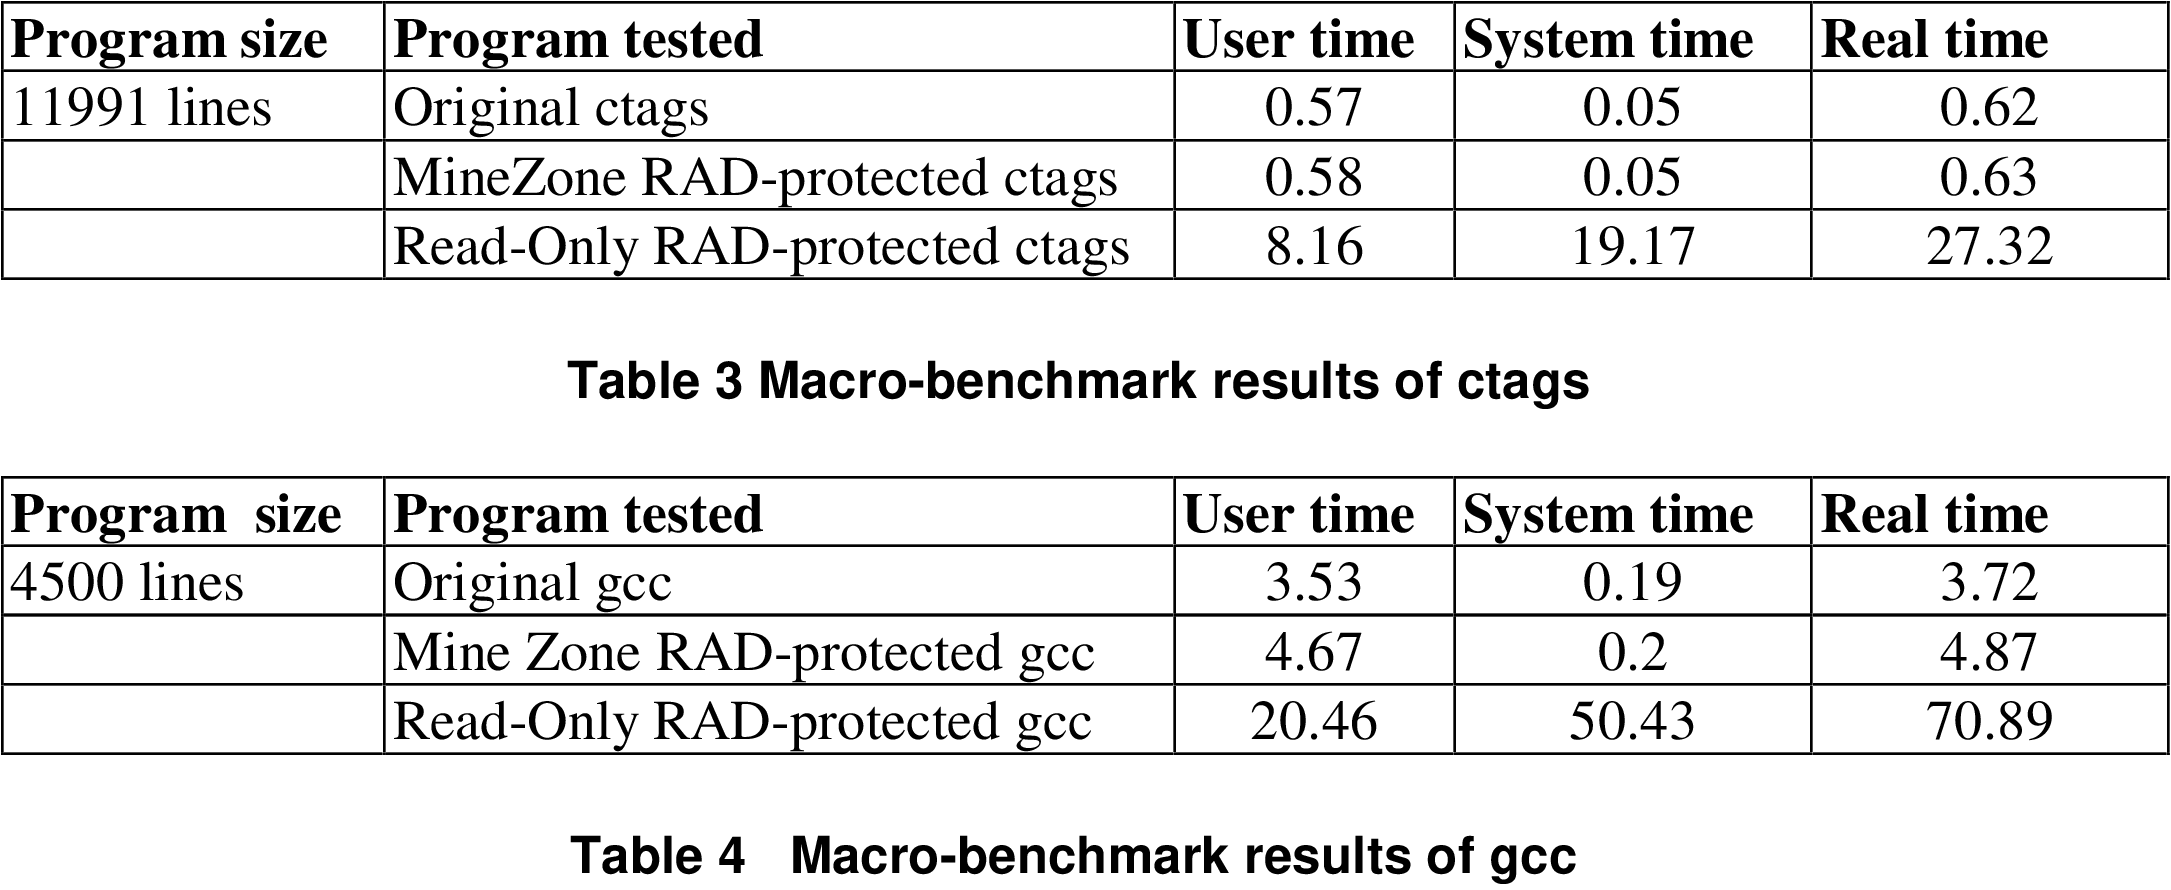
\includegraphics[height=0.8\textheight]{../mitigate/rad-results}
\end{frame}



\subsection{exceptions, setjmp, etc.}
\usetikzlibrary{arrows.meta,patterns}

\begin{frame}{automatic shadow stacks?}
    \begin{itemize}
    \item if we change how CALL/RET works\ldots
    \item \ldots maybe we can add shadow stack support to existing programs?
    \begin{itemize}
        \item either with hardware support, or
        \item in software with emulation techniques?
        \end{itemize}
    \vspace{.5cm}
    \item well, there's a problem\ldots
    \end{itemize}
\end{frame}


\begin{frame}[fragile,label=noAutomaticStack1]{the problem in C++}
\begin{lstlisting}[language=C++,style=smaller]
void Foo() {
    try {
        ... Bar() ...
    } except (std::runtime_error &error) {
        ...
    }
}

void Bar() {
    ... Quux() ...
}
void Quux() {
    ...
    throw std::runtime_error("...");
    ...
}
\end{lstlisting}    
\end{frame}

\begin{frame}[fragile,label=noAutomaticStack2]{the problem in C}
\begin{lstlisting}[language=C++,style=smaller]
jmp_buf env;
const char *error;
void Foo() {
    if (0 == setjmp(env)) {
        Bar();
    } else {
        ...
    }
}

void Bar() {
    ... Quux() ...
}
void Quux() {
    ...
    error = "...";
    longjmp(env, 1);
    ...
}
\end{lstlisting}    
\end{frame}

\begin{frame}{shadow stacks and non-lcoal returns}
    \begin{itemize}
    \item need to modify these functions to support shadow stacks, it seems?
    \item violates idea of hardware extension that modifies CALL/RET operation
    \end{itemize}
\end{frame}

\begin{frame}{one way: dealing with non-local returns}
\begin{itemize}
\item exceptions and setjmp/longjmp deliberately skip return calls
\item one solution: ``direct'' shadow stack
\item fixed (possibly secret) offset from normal stack
\item shadow stack only stores return addreses
    \begin{itemize}
    \item space in between return addresses left as nulls
    \end{itemize}
\end{itemize}
\begin{tikzpicture}[overlay,remember picture]
\coordinate (top) at ([xshift=-5cm,yshift=-2.5cm]current page.north east);
\draw[very thick] (top) rectangle ++(4cm, -7cm);
\draw[thick,pattern=north west lines] (top) ++(0cm, -1cm) rectangle ++(4cm, -2cm) node[yshift=-0.5cm,midway,fill=white] {shadow stack};
\draw[thick,pattern=north west lines] (top) ++(0cm, -4cm) rectangle ++(4cm, -2cm) node[yshift=-0.5cm,midway,fill=white] {normal stack};
\draw[thick,fill=blue!20] (top) ++(0cm, -1.4cm) rectangle  ++(4cm, -0.1cm) coordinate (after shadow ra);
\draw[thick,fill=blue!20] (top) ++(0cm, -4.4cm) rectangle  ++(4cm, -0.1cm) coordinate (after ra);
\draw[thick,fill=blue!20] (top) ++(0cm, -1.1cm) rectangle  ++(4cm, -0.1cm);
\draw[thick,fill=blue!20] (top) ++(0cm, -4.1cm) rectangle  ++(4cm, -0.1cm);
\draw[thick,fill=orange!20] (top) ++(0cm, -4.2cm) rectangle  ++(4cm, -0.2cm);
\draw[thick,fill=orange!20] (top) ++(0cm, -4cm) rectangle  ++(4cm, -0.1cm);
\node[anchor=north,font=\small,fill=white] at ([xshift=-2cm]after shadow ra) {shadow RA};
\node[anchor=north,font=\small,fill=white] at ([xshift=-2cm]after ra) {return addr};
\path[draw,very thick,-Latex] (after ra) -- ++(.25cm,0cm) |- (after shadow ra);
\end{tikzpicture}
\end{frame}


\subsection{exercise: shadow stacks stop}
\begin{frame}{what do shadow stacks stop?}
    \begin{itemize}
    \item combined with a information leak that can dump arbitrary bytes of memory, \\
       which of these exploits would shadow stacks stop\ldots
    \begin{itemize}
    \item A. using format string exploit to point stack return address to the `system' function
    \item B. using format string exploit to point VTable to the `system' function
    \item C. using an unchecked string copy that goes over the end of a stack buffer into the return address and pointing the return address to the `system' function
    \item D. using a buffer overflow that overwrites a saved stack pointer value to cause return to use a different address
    \item E. using pointer subterfuge to overwrite the GOT entry for `printf' to point to the `system' function
    \end{itemize}
    \end{itemize}
\end{frame}


\subsection{pointer subterfuge}
\usetikzlibrary{calc}
\begin{frame}[fragile,label=pointerSub]{pointer subterfuge}
\lstset{
    language=C,
    style=small,
    moredelim={**[is][\btHL<2|handout:0>]{~2~}{~end~}},
    morekeywords={size_t},
}
\begin{lstlisting}
void f2b(void *arg, size_t len) {
    char buffer[100];
    long val = ...; /* assume on stack */
    long *ptr = ...; /* assume on stack */
    memcpy(buff, arg, len); /* overwrite ptr? */
    ~2~*ptr = val~end~; /* arbitrary memory write! */
}
\end{lstlisting}
\imagecredit{adapted from Pincus and Baker, Figure 2}
% FIXME: stack picture
\end{frame}





\subsection{example: return address overwrite}
\usetikzlibrary{arrows.meta}
\begin{frame}[fragile,label=skipCanary]{skipping the canary}
\begin{tikzpicture}
% FIXME:
\tikzset{
    stackBox/.style={very thick},
    onStack/.style={thick},
}
\begin{scope}[xscale=1.2]
\draw[stackBox] (0, 0) rectangle (10, -6);
\draw[thick,-Latex] (10.25,-5) -- (10.25, -1) node [midway, below, sloped] {increasing addresses};
\node[at={(5, 0.1)},anchor=south] { highest address (stack started here)};
\node[at={(5, -6.1)},anchor=north] { lowest address (stack grows here)};

\draw[onStack] (0, -.25) rectangle (10, -1.25) node[midway,align=center,font=\small] (stackAddr)
     {return address for {\tt f2b} };
\draw[onStack,fill=red!20] (0, -1.25) rectangle (10, -2.25) node[midway,align=center,font=\small] (canaryAddr)
     {stack canary};
\draw[onStack,fill=green!20] (0, -2.25) rectangle (10, -2.75) node[midway,align=center,font=\small] (ptr) {ptr (8 bytes)};
\draw[onStack,fill=green!20] (0, -2.75) rectangle (10, -3.25) node[midway,align=center,font=\small] (val) {val (8 bytes)};
\draw[onStack,fill=blue!20] (0, -3.25) rectangle (10, -5.25) node[midway,align=center,font=\small] {buffer (100 bytes)};

\draw[onStack] (0, -5.25) rectangle (10, -6) node[midway,align=center,font=\small] {return address for {\tt scanf}};

\begin{visibleenv}<2->
\draw[-Latex,orange,ultra thick] ([xshift=1cm]ptr.east) -- ++(2cm,0cm) |- (stackAddr.east);
\draw[-Latex,orange,ultra thick,dashed] ([xshift=1cm]val.east) -- ++(2cm,0cm) |- (0.25, -5);
\end{visibleenv}

\begin{visibleenv}<3>
\draw[-Latex,red,ultra thick] ([yshift=2.5mm]stackAddr.south east) -- ++(.25cm,0cm) |- (0.25, -5);
\node[anchor=south west,red] at (0.25, -4.75) {
    machine code for the attacker to run
};
\end{visibleenv}
\end{scope}
\end{tikzpicture}
\end{frame}


\section{beyond stack smashing}
\begin{frame}{beyond return addresses}
    \begin{itemize}
    \item pointer subterfuge let us overwrite anything
    \item my example: showed return address
    \item but return address is tricky to locate exactly
    \item but there are \myemph{easier options!}
    \end{itemize}
\end{frame}


\section{arbitrary writes}

\begin{frame}<1-3>[label=arbWrite]{arbitrary memory write}
    \begin{itemize}
    \item bunch of scenarios that lead to \myemph{single arbitrary memory write}
        \begin{itemize}
        \item format exploits are one, but we'll find more!!
        \end{itemize}
    \item typical result: arbitrary code execution
    \item how?
    \vspace{.5cm}
    \item<2-> \myemph<3>{overwrite existing machine code (insert jump?)}
        \begin{itemize}
        \item problem: usually not writable
        \end{itemize}
    \item<2-> \myemph<4>{overwrite return address directly}
        \begin{itemize}
        \item observation: don't care about stack canaries --- skip them
        \end{itemize}
    \item<2-> \myemph<5>{overwrite other function pointer?}
    \item<2-> \myemph<6>{overwrite another data pointer --- copy more?}
    \end{itemize}
\end{frame}


\section{write targets, continued}

\subsection{C++ inheritence}
\usetikzlibrary{arrows.meta,matrix}

\begin{frame}[fragile,label=CPPVirt]{C++ inheritence}
\lstset{
    language=C++,style=smaller,
}
\begin{lstlisting}
class InputStream {
public:
    virtual int get() = 0;
    // Java: abstract int get();
    ...
};
class SeekableInputStream : public InputStream {
public:
    virtual void seek(int offset) = 0;
    virtual int tell() = 0;
};
class FileInputStream : public InputStream {
public:
    int get();
    void seek(int offset);
    int tell();
    ...
};
\end{lstlisting}
\end{frame}

\begin{frame}<1>[label=inheritMemLay]{C++ inheritence: memory layout}
\begin{tikzpicture}
    \tikzset{
        vt/.style={fill=blue!30},
    }
    \matrix[tight matrix,nodes={text width=3.8cm,text depth=.1ex,font=\small\tt},
            label={north:InputStream},anchor=north west] (inputStream)  at (0, 0) {
        |[vt]| vtable pointer \\
    };
    \matrix[tight matrix,nodes={text width=3.8cm,text depth=.1ex,font=\small\tt},
            label={north:SeekableInputStream},anchor=north west] (seekableStream) at (4.5, 0) {
        |[vt]| vtable pointer \\
    };
    \matrix[tight matrix,nodes={text width=6cm,text depth=.1ex,font=\small\tt},
            label={north:FileInputStream},anchor=north west] (fileStream) at (9, 0) {
        |[vt]| vtable pointer \\
        file\_pointer \\
    };
    \matrix[tight matrix,nodes={text width=3.8cm,text depth=.1ex,font=\small\tt},anchor=north west] (isVT) at (0, -2) {
        \tt slot for get\\
    };
    \matrix[tight matrix,nodes={text width=3.8cm,text depth=.1ex,font=\small\tt},anchor=north west] (seekVT) at (4.5, -2){
        \tt slot for get \\
        \tt slot for seek \\
        \tt slot for tell \\
    };
    \matrix[tight matrix,nodes={text width=6cm,text depth=.1ex,font=\small\tt},anchor=north west] (fileVT) at (9, -2){
        FileInputStream::get \\
        FileinputStream::seek \\
        FileInputStream::tell \\
    };
    \draw[thick,-Latex] (inputStream-1-1.east) -- ++(.35cm,0cm) |- (isVT-1-1.east);
    \draw[thick,-Latex] (seekableStream-1-1.east) -- ++(.35cm,0cm) |- (seekVT-1-1.east);
    \draw[thick,-Latex] (fileStream-1-1.east) -- ++(.35cm,0cm) |- (fileVT-1-1.east);
\end{tikzpicture}
\end{frame}

\begin{frame}[fragile,label=CPPImpl]{C++ implementation (pseudo-code)}
\lstset{
    language=C,style=smaller,
}
\begin{lstlisting}
struct InputStream_vtable {
    int (*get)(InputStream* this);
};

struct InputStream {
    InputStream_vtable *vtable;
};

...

    InputStream *s = ...;
    int c = (s->vtable->get)(s);
\end{lstlisting}
\end{frame}

\begin{frame}[fragile,label=CPPImplB]{C++ implementation (pseudo-code)}
\lstset{
    language=C,style=smaller,
}
\begin{lstlisting}
struct SeekableInputStream_vtable {
    struct InputStream_vtable as_InputStream;
    void (*seek)(SeekableInputStream* this, int offset);
    int (*tell)(SeekableInputStream* this);
};

struct FileInputStream {
    SeekableInputStream_vtable *vtable;
    FILE *file_pointer;
};

...

    FileInputStream file_in = { the_FileInputStream_vtable,  ... };
    InputStream *s = (InputStream*) &file_in;
\end{lstlisting}
\end{frame}

\begin{frame}[fragile,label=CPPImplC]{C++ implementation (pseudo-code)}
\lstset{
    language=C,style=smaller,
}
\begin{lstlisting}
SeekableInputStream_vtable the_FileInputStream_vtable = {
    &FileInputStream_get,
    &FileInputStream_seek,
    &FileInputStream_tell,
};

...

    FileInputStream file_in = { the_FileInputStream_vtable,  ... };
    InputStream *s = (InputStream*) &file_in;
\end{lstlisting}
\end{frame}




\subsection{options for attacking function pointer tables}
    % FIXME: find another function pointer in memory

\begin{frame}{attacking function pointer tables}
% FIXME: picture
\begin{itemize}
\item option 1: overwrite table entry directly  
    \begin{itemize}
    \item required/easy for Global Offset Table --- fixed location
    \item usually not possible for VTables --- read-only memory
    \end{itemize}
\item option 2: create table in buffer (big list of pointers to shellcode), point to buffer
    \begin{itemize}
    \item useful when table pointer next to buffer
    \item (e.g. C++ object on stack next to buffer)
    \end{itemize}
\item option 3: find suitable pointer elsewhere
    \begin{itemize}
    \item e.g. point to wrong part of vtable to run different function
    \end{itemize}
\end{itemize}
\end{frame}




\subsection{vtable overwrite exercise}
\usetikzlibrary{arrows.meta,matrix}
\begin{frame}[fragile,label=vtExer]{exercise}
\vspace{-.25cm}
\begin{tikzpicture}
    \tikzset{
        vt/.style={fill=blue!30},
    }
    \matrix[tight matrix,nodes={text width=3.8cm,text depth=.1ex,font=\small\tt},
            label={north:objArray},anchor=north west] (vulnClass)  at (0, 0) {
        |[vt]| vtable pointer \\
        |[minimum height=1cm]| buffer\\
        |[vt]| vtable pointer \\
        |[minimum height=1cm]| \ldots \\
    };
    \matrix[tight matrix,nodes={text width=3.8cm,text depth=.1ex,font=\small\tt},anchor=north west] (isVT) at (0, -3) {
        \tt slot for foo\\
        \tt slot for bar\\
    };
    \draw[thick,-Latex] (vulnClass-1-1.east) -- ++(.45cm,0cm) |- (isVT-1-1.east);
    \draw[thick,-Latex] (vulnClass-3-1.east) -- ++(.35cm,0cm) |- (isVT-1-1.east);
    \node[anchor=north west] at (5, 0) {
\begin{lstlisting}[language=C++,style=smaller]
class VulnerableClass {
public:
    char buffer[100];
    virtual void foo();
    virtual void bar();
};
VulnerableClass objArray[10];
\end{lstlisting}
};
\end{tikzpicture}
\begin{itemize}
\item if we can overflow \texttt{objArray[0].buffer} to change array[1]'s vtable pointer and know array[1].foo() will be called; finish the plan:
\end{itemize}
\small \begin{tabular}{ll}
buffer[0]: \rule{2cm}{.1mm} \hspace{1cm} & A. shellcode \\
buffer[50]: \rule{2cm}{.1mm} \hspace{1cm} & B. address of buffer[0]\\
array[1]'s vtable pointer: \rule{2cm}{.1mm} \hspace{1cm} & C. address of buffer[50] \\
~ & D. address of original vtable \\
~ & E. address of objArray[0]'s vtable \\
~ & E. address of objArray[1]'s vtable pointer \\
\end{tabular}
\end{frame}


\section{one write into another}
\againframe<6>{arbWrite}


\subsection{example: GOT overwrite}

\begin{frame}[fragile,label=gotOverwrite]{attacking the GOT}
\begin{tikzpicture}
% FIXME:
\tikzset{
    stackBox/.style={very thick},
    onStack/.style={thick},
}
\draw[stackBox] (0, 0) rectangle (10, -6);
\draw[thick,-Latex] (10.25,-5) -- (10.25, -1) node [midway, below, sloped] {increasing addresses};
\node[at={(5, 0.1)},anchor=south] { highest address (stack started here)};
\node[at={(5, -6.1)},anchor=north] { lowest address (stack grows here)};

\draw[onStack] (0, -.25) rectangle (10, -1.25) node[midway,align=center,font=\small] (stackAddr)
     {return address for {\tt f2b} };
\draw[onStack,fill=red!20] (0, -1.25) rectangle (10, -2.25) node[midway,align=center,font=\small] (canaryAddr)
     {stack canary};
\draw[onStack,fill=green!20] (0, -2.25) rectangle (10, -2.75) node[midway,align=center,font=\small] (ptr) {ptr (8 bytes)};
\draw[onStack,fill=green!20] (0, -2.75) rectangle (10, -3.25) node[midway,align=center,font=\small] (val) {val (8 bytes)};
\draw[onStack,fill=blue!20] (0, -3.25) rectangle (10, -5.25) node[midway,align=center,font=\small] {buffer (100 bytes)};

\draw[onStack] (0, -5.25) rectangle (10, -6) node[midway,align=center,font=\small] {return address for {\tt scanf}};

\node[anchor=south] at (13.5, -1) { global offset table };
\draw[stackBox] (11.5, -1) rectangle (15.25, -1.5) node[midway,font=\small] (printfEntry) {GOT entry: printf };
\draw[stackBox] (11.5, -1.5) rectangle (15.25, -2) node[midway,font=\small] {GOT entry: fopen };
\draw[stackBox] (11.5, -2) rectangle (15.25, -2.5) node[midway,font=\small] {GOT entry: exit };

\begin{visibleenv}<2->
\draw[-Latex,orange,ultra thick] ([xshift=1cm]ptr.east) -- ++(2cm,0cm) |- (printfEntry.west);
\draw[-Latex,orange,ultra thick,dashed] ([xshift=1cm]val.east) -- ++(2cm,0cm) |- (0.25, -5);
\end{visibleenv}

\begin{visibleenv}<3>
\draw[-Latex,red,ultra thick] ([yshift=2.5mm]printfEntry.south east) -- ++(.25cm,0cm) |- (0.25, -5);
\node[anchor=south west,red,inner sep=0.1mm] at (0.25, -4.75) {
    machine code for the attacker to run
};
\end{visibleenv}
\end{tikzpicture}
\end{frame}



\subsubsection{careful stack layout?}
\begin{frame}{laying out stack to avoid subterfuge (1)}
\begin{tikzpicture}
% FIXME:
\tikzset{
    stackBox/.style={very thick},
    onStack/.style={thick},
}
\begin{scope}[xscale=1.2]
\draw[stackBox] (0, 0) rectangle (10, -6);
\draw[thick,-Latex] (10.25,-5) -- (10.25, -1) node [midway, below, sloped] {increasing addresses};
\node[at={(5, 0.1)},anchor=south] { highest address (stack started here)};
\node[at={(5, -6.1)},anchor=north] { lowest address (stack grows here)};

\draw[onStack] (0, -.25) rectangle (10, -1.25) node[midway,align=center,font=\small] (stackAddr)
     {return address for {\tt vulnerable} };
\draw[onStack,fill=red!20] (0, -1.25) rectangle (10, -2.25) node[midway,align=center,font=\small] (canaryAddr)
     {stack canary};
\draw[onStack,fill=blue!20] (0, -2.25) rectangle (10, -4.25) node[midway,align=center,font=\small] {buffer (100 bytes)};

\draw[onStack,fill=green!20] (0, -4.25) rectangle (10, -4.75) node[midway,align=center,font=\small] (ptr) {array (8 bytes)};
\draw[onStack] (0, -4.75) rectangle (10, -5.5) node[midway,align=center,font=\small] {return address for {\tt gets}};

\end{scope}
\end{tikzpicture}
\end{frame}

\begin{frame}{laying out stack to avoid subterfuge (2)}
\begin{tikzpicture}
% FIXME:
\tikzset{
    stackBox/.style={very thick},
    onStack/.style={thick},
}
\begin{scope}[xscale=1.2]
\draw[stackBox] (0, 0) rectangle (10, -6);
\draw[thick,-Latex] (10.25,-5) -- (10.25, -1) node [midway, below, sloped] {increasing addresses};
\node[at={(5, 0.1)},anchor=south] { highest address (stack started here)};
\node[at={(5, -6.1)},anchor=north] { lowest address (stack grows here)};

\draw[onStack] (0, -.25) rectangle (10, -1.25) node[midway,align=center,font=\small] (stackAddr)
     {return address for {\tt f2b} };
\draw[onStack,fill=red!20] (0, -1.25) rectangle (10, -2.25) node[midway,align=center,font=\small] (canaryAddr)
     {stack canary};
\draw[onStack,fill=blue!20] (0, -2.25) rectangle (10, -4.25) node[midway,align=center,font=\small] {buffer (100 bytes)};

\draw[onStack,fill=green!20] (0, -4.25) rectangle (10, -4.75) node[midway,align=center,font=\small] (ptr) {ptr (8 bytes)};
\draw[onStack,fill=green!20] (0, -4.75) rectangle (10, -5.25) node[midway,align=center,font=\small] (val) {val (8 bytes)};
\draw[onStack] (0, -5.25) rectangle (10, -6) node[midway,align=center,font=\small] {return address for {\tt scanf}};

\end{scope}
\end{tikzpicture}
\end{frame}



\subsubsection{structs containing pointers}
\usetikzlibrary{arrows.meta}
\begin{frame}[fragile,label=structSubter]{other subterfuge cases (1)}
\begin{lstlisting}[language=C,style=small]
struct Command {
  CommandType type;
  int values[MAX_VALUES];
  int *active_value;
  ...
};
\end{lstlisting}
\begin{tikzpicture}[overlay,remember picture]
% FIXME:
\tikzset{
    stackBox/.style={very thick},
    onStack/.style={thick},
}
\coordinate (my anchor) at ([xshift=-9cm,yshift=-2cm]current page.north east);
\begin{scope}[shift={(my anchor)},xscale=0.8]
\draw[stackBox] (0, 0) rectangle (10, -6);
\draw[thick,-Latex] (10.25,-5) -- (10.25, -1) node [midway, below, sloped] {increasing addresses};
\node[at={(5, 0.1)},anchor=south] { highest address };
\node[at={(5, -6.1)},anchor=north] { lowest address };

\draw[onStack] (0, -.25) rectangle (10, -2.25) node[midway,align=center,font=\small] (stackAddr)
     {more struct fields};
\draw[onStack,fill=green!20] (0, -2.25) rectangle (10, -2.75) node[midway,align=center,font=\small] (ptr) {active\_value};
\draw[onStack,fill=blue!20] (0, -2.75) rectangle (10, -5.25) node[midway,align=center,font=\small] {values};
\draw[onStack,fill=yellow!20] (0, -5.25) rectangle (10, -5.75) node[midway,align=center,font=\small] {type};
\end{scope}
\end{tikzpicture}
\end{frame}

\begin{frame}[fragile,label=globalSubter]{other subterfuge cases (2)}
\begin{lstlisting}[language=C,style=small]
Command *current_command;
char input_buffer[4096];

void run_next_command() {
  if (!current_command) {
    current_command =
        getNext();
  }
  current_command-> ...
  ...
}
\end{lstlisting}
\begin{tikzpicture}[overlay,remember picture]
% FIXME:
\tikzset{
    stackBox/.style={very thick},
    onStack/.style={thick},
}
\coordinate (my anchor) at ([xshift=-9cm,yshift=-2cm]current page.north east);
\begin{scope}[shift={(my anchor)},xscale=0.8]
\draw[stackBox] (0, 0) rectangle (10, -6);
\draw[thick,-Latex] (10.25,-5) -- (10.25, -1) node [midway, below, sloped] {increasing addresses};
\node[at={(5, 0.1)},anchor=south] { highest address };
\node[at={(5, -6.1)},anchor=north] { lowest address };

\draw[onStack] (0, -.25) rectangle (10, -2.25) node[midway,align=center,font=\small] (stackAddr)
     {more globals};
\draw[onStack,fill=green!20] (0, -2.25) rectangle (10, -2.75) node[midway,align=center,font=\small] (ptr) {current\_command};
\draw[onStack,fill=blue!20] (0, -2.75) rectangle (10, -5.25) node[midway,align=center,font=\small] {input\_buffer};
\draw[onStack] (0, -5.25) rectangle (10, -5.75) node[midway,align=center,font=\small] {more globals};
\end{scope}
\end{tikzpicture}
\end{frame}


\section{arc injection}
\begin{frame}{so far overwrites}
    \begin{itemize}
    \item once we found a way to overwrite function pointer\\
          easiest solution seems to be: direct to our code
    \item \ldots but alterante places to direct it to
    \end{itemize}
\end{frame}

\usetikzlibrary{arrows.meta}

\begin{frame}[fragile,label=returnToSomewhere]{return-to-somewhere}
\begin{tikzpicture}
% FIXME:
\tikzset{
    stackBox/.style={very thick},
    onStack/.style={thick},
}
\begin{scope}[xscale=0.75]
\draw[stackBox] (0, 0) rectangle (10, -6);
\draw[thick,-Latex] (10.25,-5) -- (10.25, -1) node [midway, below, sloped] {increasing addresses};
\node[at={(5, 0.1)},anchor=south] { highest address (stack started here)};
\node[at={(5, -6.1)},anchor=north] { lowest address (stack grows here)};

\draw[onStack] (0, -.25) rectangle (10, -1.25) node[midway,align=center,font=\small] (stackAddr)
     {return address for {\tt vulnerable}: \\ address of {\tt do\_useful\_stuff}};
\draw[onStack,fill=black!20] (0, -1.25) rectangle (10, -2.25) node[midway,align=center,font=\small] {unused space (20 bytes)};
\draw[onStack,fill=blue!20] (0, -2.25) rectangle (10, -5.25) node[midway,align=center,font=\small] {buffer (100 bytes)};

\draw[onStack] (0, -5.25) rectangle (10, -6) node[midway,align=center,font=\small] {return address for {\tt scanf}};

\draw[onStack,fill=red!20,opacity=0.9] (0, -5.25) rectangle (10, -1.25) node[midway,align=center,font=\small,text=red!50!black] {unused junk};

\draw[-Latex,red,ultra thick,dashed] ([yshift=2.5mm]stackAddr.south east) -- ++(.25cm,0cm) |-
    (11, -4.25) node[align=left,right,font=\small] { {\tt do\_useful\_stuff} \\ (already in program) };

\begin{visibleenv}<2>
\fill[white,opacity=0.5, overlay] (-1,-2) rectangle (18, -8);
\end{visibleenv}
\end{scope}
\end{tikzpicture}
\begin{tikzpicture}[overlay,remember picture]
\begin{visibleenv}<2>
\node[fill=white,draw,ultra thick,align=center,anchor=center] at (current page.center) {
    code is \myemph{already in program}??? \\
    how often does this happen??? \\
    \ldots turns out ``\myemph{usually}'' --- more later in semester
};
\end{visibleenv}
\end{tikzpicture}
\end{frame}

\begin{frame}[fragile,label=systemFunc]{example: system()}
\begin{lstlisting}[language={}]
NAME
       system - execute a shell command

SYNOPSIS
       #include <stdlib.h>

       int system(const char *command);
\end{lstlisting}
\begin{itemize}
\item part of C standard library
\item in any program that dynamically links to libc
\item challenge: need to hope argument register (rdi) set usefully
\end{itemize}
\end{frame}

\begin{frame}[fragile,label=locateSystem]{locating system() Linux}
\begin{lstlisting}[language={},style=script,
moredelim={**[is][\btHL<1>]{~1~}{~end~}},
]
$ ldd /bin/ls
        linux-vdso.so.1 (0x00002aaaaaade000)
        libselinux.so.1 => /lib/x86_64-linux-gnu/libselinux.so.1 (0x00002aaaaab3a000)
        libc.so.6 => /lib/x86_64-linux-gnu/libc.so.6 (~1~0x00002aaaaab65000~end~)
        libpcre2-8.so.0 => /usr/lib/x86_64-linux-gnu/libpcre2-8.so.0 (0x00002aaaaad57000)
        libdl.so.2 => /lib/x86_64-linux-gnu/libdl.so.2 (0x00002aaaaade7000)
        /lib64/ld-linux-x86-64.so.2 (0x00002aaaaaaab000)
        libpthread.so.0 => /lib/x86_64-linux-gnu/libpthread.so.0 (0x00002aaaaaded000)
$ objdump --dynamic-syms /lib/x86_64-linux-gnu/libc.so.6 | grep system
0000000000156a80 g    DF .text  0000000000000067  GLIBC_2.2.5 svcerr_systemerr
0000000000055410 g    DF .text  000000000000002d  GLIBC_PRIVATE __libc_system
~1~0000000000055410~end~  w   DF .text  000000000000002d  GLIBC_2.2.5 system
\end{lstlisting}
\begin{itemize}
\item if address randomization disabled: \\
address should be 0x00002aaaaab650 + 0x55410
\vspace{.5cm}
\item \texttt{ldd} --- ``what libraries does this load and where?''
    \begin{itemize}
    \item similar tools for other OSes
    \end{itemize}
\end{itemize}
\end{frame}


\section{case study: NTP exploit}
\usetikzlibrary{arrows.meta,patterns}
\begin{frame}[fragile,label=ntpStudyIntro]{case study (simplified)}
    \begin{itemize}
    \item bug in NTPd (Network Time Protocol Daemon)
    \item via Stephen R\"ottger, ``Finding and exploiting ntpd vulnerabilities''
        \begin{itemize}
        \item \url{https://googleprojectzero.blogspot.com/2015/01/finding-and-exploiting-ntpd.html}
        \end{itemize}
    \end{itemize}
\lstset{
    language=C,
    style=small,
    moredelim={**[is][\btHL<1|handout:0>]{~1~}{~end~}},
    moredelim={**[is][\btHL<2|handout:0>]{~2~}{~end~}},
}
\begin{lstlisting}
static void
ctl_putdata(
  const char *dp,
  unsigned int dlen,
  int bin   /* set to 1 when data is binary */
  ) {
    ...
    ~1~memmove((char *)datapt, dp, (unsigned)dlen);~end~
    datapt += dlen;
    datalinelen += dlen;
}
\end{lstlisting}
\end{frame}

\begin{frame}<1>[fragile,label=target]{the target}
\lstset{
    language=C,
    style=small,
    moredelim={**[is][\btHL<1|handout:0>]{~1~}{~end~}},
    moredelim={**[is][\btHL<2|handout:0>]{~2~}{~end~}},
}
\begin{lstlisting}
    memmove((char *)~1~datapt~end~, dp, (unsigned)dlen);
\end{lstlisting}
\begin{tikzpicture}
\tikzset{box/.style={thick}}
\draw[box,fill=blue!20] (0, 0) rectangle (10, -0.5) node[midway] (datapt) {datapt (global variable)};
\draw[box,fill=green!20] (0, -0.5) rectangle (10, -1.5) node[midway] {(other global variables)};
\draw[box,fill=red!20] (0, -1.5) rectangle (10, -2.5) node[midway] (buffer) {buffer (global array)};
\begin{visibleenv}<1-2>
    \draw[very thick,violet!70!black,-Latex] (datapt.west) -- ++(-.5cm,0cm) -| (0.5, -1.75);
\end{visibleenv}
\begin{visibleenv}<2->
    \draw[box,fill=orange!20] (11, -1) rectangle (15, -1.5) node[midway] (strlen) {strlen GOT entry};
\end{visibleenv}
\begin{visibleenv}<3->
    \fill[pattern=north west lines,pattern color=red,opacity=0.4] (0, -2.5) rectangle (10, 0);
    \draw[-Latex,very thick,dashed,red] (datapt) -| ([xshift=-0.5cm]strlen.west) -- (strlen.west);
\end{visibleenv}
\begin{visibleenv}<4->
    \draw[box,fill=violet!20] (11, -3) rectangle (15, -3.5) node[midway] (system) {{\tt system()} stub};
    \fill[pattern=north west lines,pattern color=red,opacity=0.4] (11, -1) rectangle (15, -1.5);
    \draw[-Latex,very thick,dashed,red] (strlen.south) -- (system.north);
\end{visibleenv}
\end{tikzpicture}
\end{frame}

\begin{frame}[fragile,label=moreContext]{more context}
\lstset{
    language=C,
    moredelim={**[is][\btHL<1|handout:0>]{~1~}{~end~}},
    moredelim={**[is][\btHL<2|handout:0>]{~2~}{~end~}},
}
\begin{lstlisting}
    memmove((char *)~1~datapt~end~, dp, (unsigned)dlen);
    ...
    ...
    strlen(some_user_supplied_string)
    /* calls strlen@plt
       looks up global offset table entry! */
\end{lstlisting}
\end{frame}

\againframe<2>{target}

\begin{frame}{overall exploit}
    \begin{itemize}
    \item overwrite {\tt datapt} to point to strlen GOT entry
    \item overwrite value of strlen GOT entry
    \item example target: {\tt system} function
            \begin{itemize}
                \item executes command-line command specified by argument
            \end{itemize}
    \item supply string to provide argument to ``{\tt strlen}''
    \end{itemize}
\end{frame}

\againframe<3->{target}

\begin{frame}{overall exploit: reality}
    \begin{itemize}
    \item real exploit was more complicated
    \item needed to defeat more mitigations
    \item needed to deal with not being able to write {\tt \textbackslash 0}
    \item actually tricky to send things that trigger buffer write
        \begin{itemize}
        \item (meant to be local-only)
        \end{itemize}
    \end{itemize}
\end{frame}



\subsection{subterfuge exercise}
\begin{frame}[fragile,label=subterExer]{subterfuge exercise}
\begin{lstlisting}[language=C++,style=script]
struct Student {
    char email[128];
    struct Assignment *assignments[16];
    ...
};
struct Assignment {
    char submission_file[128];
    char regrade_request[1024];
    ...
};
void SetEmail(Student *s, char *new_email) { strcpy(s->email, new_email); }
void AddRegradeRequest(Student *s, int index, char *request) {
    strcpy(s->assignments[index]->regrade_request, request);
}
void vulnerable(char *STRING1, char *STRING2) {
    SetEmail(s, STRING1); AddRegradeRequest(s, 0, STRING2);
}
\end{lstlisting}
\begin{itemize}
\item exercise: to set \texttt{0x1020304050} to \texttt{0xAABBCCDD}, what should STRING1, STRING2 be?
    \begin{itemize}
    \item (assume 64-bit pointers, no padding in structs, little-endian)
    \end{itemize}
\end{itemize}
\end{frame}



\section{backup slides}
\begin{frame}{backup slides}
\end{frame}

\end{document}
